%  LaTeX support: latex@mdpi.com
%  In case you need support, please attach all files that are necessary for compiling as well as the log file, and specify the details of your LaTeX setup (which operating system and LaTeX version / tools you are using).

% You need to save the "mdpi.cls" and "mdpi.bst" files into the same folder as this template file.

%=================================================================
\documentclass[sensors,article,submit,moreauthors,pdftex,10pt,a4paper]{mdpi}
%
%--------------------
% Class Options:
%--------------------
% journal
%----------

% article
%---------
% The default type of manuscript is article, but can be replaced by:
% addendum, article, benchmark, book, bookreview, briefreport, casereport, changes, comment, commentary, communication, conceptpaper, correction, conferenceproceedings, conferencereport, expressionofconcern, meetingreport, creative, datadescriptor, discussion, editorial, essay, erratum, hypothesis, interestingimages, letter, newbookreceived, opinion, obituary, projectreport, reply, reprint, retraction, review, perspective, preprints, protocol, shortnote, supfile, technicalnote, viewpoint
% supfile = supplementary materials
% protocol: If you are preparing a "Protocol" paper, please refer to http://www.mdpi.com/journal/mps/instructions for details on its expected structure and content.
%----------
% submit
%----------
% The class option "submit" will be changed to "accept" by the Editorial Office when the paper is accepted. This will only make changes to the frontpage (e.g. the logo of the journal will get visible), the headings, and the copyright information. Also, line numbering will be removed. Journal info and pagination for accepted papers will also be assigned by the Editorial Office.
%------------------
% moreauthors
%------------------
% If there is only one author the class option oneauthor should be used. Otherwise use the class option moreauthors.
%---------
% pdftex
%---------
% The option pdftex is for use with pdfLaTeX. If eps figure are used, remove the option pdftex and use LaTeX and dvi2pdf.
\usepackage{amssymb}
\usepackage{amsmath}
\usepackage{epstopdf}
\usepackage{hyperref}
\usepackage{color}
\usepackage{multirow}
\usepackage{subcaption}

%=================================================================
\newcommand{\ml}[1]{\textcolor{blue}{ Mathieu: #1}}
\newcommand{\fg}[1]{\textcolor{red}{ Felix: #1}}
\newcommand{\ac}[1]{\textcolor{red}{ Arnaud: #1}}
\newcommand{\pa}[1]{\textcolor{red}{ Pierre: #1}}
\newcommand{\cl}[1]{\textcolor{red}{ Catherine: #1}}
\firstpage{1}
\makeatletter
\setcounter{page}{\@firstpage}
\makeatother
\articlenumber{x}
\doinum{10.3390/------}
\pubvolume{xx}
\pubyear{2017}
\copyrightyear{2017}
\history{Received: date; Accepted: date; Published: date}

%------------------------------------------------------------------
% The following line should be uncommented if the LaTeX file is uploaded to arXiv.org
%\pdfoutput=1

%=================================================================
% Add packages and commands here. The following packages are loaded in our class file: fontenc, calc, indentfirst, fancyhdr, graphicx, lastpage, ifthen, lineno, float, amsmath, setspace, enumitem, mathpazo, booktabs, titlesec, etoolbox, amsthm, hyphenat, natbib, hyperref, footmisc, geometry, caption, url, mdframed, tabto, soul, multirow, microtype, tikz

%=================================================================
%% Please use the following mathematics environments: Theorem, Lemma, Corollary, Proposition, Characterization, Property, Problem, Example, ExamplesandDefinitions, Hypothesis, Remark, Definition
%% For proofs, please use the proof environment (the amsthm package is loaded by the MDPI class).

%=================================================================
% Full title of the paper (Capitalized)
\Title{An efficient audio coding scheme  for quantitative and qualitative large scale acoustic monitoring using the sensor grid approach}

% If this is an expanded version of a conference paper, please cite it here: enter the full citation of your conference paper, and add $^\dagger$ in the end of the title of this article.
%\conference{Title}


% Authors, for the paper (add full first names)
\Author{F\'elix Gontier $^{1}$, Mathieu Lagrange $^{1}$, Pierre Aumond $^{2}$, Arnaud Can $^{2}$ and Catherine Lavandier $^{3}$}

% Authors, for metadata in PDF
\AuthorNames{F\'elix Gontier, Mathieu Lagrange, Pierre Aumond, Arnaud Can and Catherine Lavandier}

% Affiliations / Addresses (Add [1] after \address if there is only one affiliation.)
\address{%
$^{1}$ \quad LS2N\\
$^{2}$ \quad IFSTTAR\\
$^{3}$ \quad Universit\'e de Cergy-Pontoise}

% Contact information of the corresponding author
\corres{Correspondence: mathieu.lagrange@cnrs.fr}



% Simple summary
%\simplesumm{}

% Abstract (Do not use inserted blank lines, i.e. \\)
\abstract{The spreading of urban areas and the growth of human population worldwide raised societal and environmental concerns. To better address those, the monitoring of the acoustic environment in urban but also rural or wilderness areas is an important matter. Fostering on the recent development of low cost hardware acoustic sensors, we propose in this paper to consider a sensor grid approach to tackle this issue. In this kind of approach, the crucial question is the nature of the data that is transmitted from the sensors to the processing and archival servers. To this end, we propose an efficient audio coding scheme based on third octave band spectral representation that allows 1) the estimation of standard acoustic indicators and 2) the recognition of acoustic events at state of the art performance rate. The former is useful to provide quantitative information about the acoustic environment, while the latter is useful to gather qualitative information and build perceptually motivated indicators using for example the emergence of a given sound source. The coding scheme is also demonstrated to transmit spectrally encoded data that, reverted to the time domain using state of the art techniques, is not intelligible, thus protecting the privacy of citizens.}

% Keywords
\keyword{acoustic monitoring; audio encoding}

% The fields PACS, MSC, and JEL may be left empty or commented out if not applicable
%\PACS{J0101}
%\MSC{}
%\JEL{}

%%%%%%%%%%%%%%%%%%%%%%%%%%%%%%%%%%%%%%%%%%
% Only for journal Applied Sciences:
%\featuredapplication{Authors are encouraged to provide a concise description of the specific application or a potential application of the work. This section is not mandatory.}
%%%%%%%%%%%%%%%%%%%%%%%%%%%%%%%%%%%%%%%%%%


%%%%%%%%%%%%%%%%%%%%%%%%%%%%%%%%%%%%%%%%%%
% Only for the journal Data:
%\dataset{DOI number or link to the deposited data set in cases where the data set is published or set to be published separately. If the data set is submitted and will be published as a supplement to this paper in the journal Data, this field will be filled by the editors of the journal. In this case, please make sure to submit the data set as a supplement when entering your manuscript into our manuscript editorial system.}

%\datasetlicense{license under which the data set is made available (CC0, CC-BY, CC-BY-SA, CC-BY-NC, etc.)}

%%%%%%%%%%%%%%%%%%%%%%%%%%%%%%%%%%%%%%%%%%
% For Conference Proceedings Papers:
%\conferencetitle{Add the conference title here}

%\setcounter{secnumdepth}{4}
%%%%%%%%%%%%%%%%%%%%%%%%%%%%%%%%%%%%%%%%%%

\begin{document}
%%%%%%%%%%%%%%%%%%%%%%%%%%%%%%%%%%%%%%%%%%
%% Only for the journal Gels: Please place the Experimental Section after the Conclusions

%%%%%%%%%%%%%%%%%%%%%%%%%%%%%%%%%%%%%%%%%%

\section{Introduction}
%\label{}

The advent of low cost acoustic sensors together with the need to better monitor and comprehend the acoustic environment of urban and wilderness areas give rise to the deployment of experimental sensor networks such as the sonyc\footnote{\url{htttp://wp.nyu.edu/sonyc}} \cite{mydlarz2017implementation} and cense\footnote{\url{htttp://cense.ifsttar.fr}} \cite{picault2017} projects. To do so, considering the so-called "sensor grid" approach  \cite{lim2005sensor,tham2005sensorgrid} has several advantages. The sensor grid approach puts the focus on a) a distributed system of data acquisition with a large set of sensors, b) the production and storage of a large dataset, and c) its availability for intensive and open data analysis computation.

In such approach,  the number of sensor nodes shall be extended as needed without having to change the hardware and software architecture, \textit{i.e.} the approach shall be scalable. Second, the nodes shall be energy efficient, ideally autonomous, in order to ease the deployment of the sensor grid to the desired topology. Third, the encoding scheme used to transmit the data from the sensor to the storage and processing servers shall be designed with care in order to ensure the privacy of the citizens. At the same time, the data stored shall remain as rich as possible while maintaining a low bitrate for efficient transmission and storage.

In the case of acoustic monitoring, the data of interest can be quantitative such as standard acoustic indicators (LAeq, ...) or qualitative such as the presence of sound sources of interest (bird calls, sirens, ...). The latter allows us to better assess the human perception of the urban sound environment in terms of pleasantness and other perceptual indicators \cite{lavandier2006contribution, aumond2017modeling}. This detection step can respectively be operated online (on the sensors) or offline (on the data servers) leading to different grid designs (Figure \ref{fig:codingScheme}).

Performing the detection online (case B of Figure \ref{fig:codingScheme}) is efficient in terms of data storage as only the detected events are transmitted. This approach is thus currently considered in several approaches in the literature \cite{defreville2006automatic, mydlarz2017implementation, mydlarz2015design}. Though, it requires the availability of decent computing resources on the sensors in order to perform the detection step which as of today's efficiency of hardware does not allow them to be autonomous using power sources like decent size solar panels. Furthermore, the detection is done once and cannot be recomputed during offline posterior analyses.

Performing the detection offline has several benefits. First, the sensor task is much simpler and can thus be implemented on low energy consumption processors, potentially being autonomous in terms of energy, which greatly ease the deployment of the network. Second, it allows researchers to gather large amount of data that can be post-processed and studied further offline. Data can be re-analyzed following newer classification schemes or using new indicators.

Though transmitting the raw audio  through the network (case A of Figure \ref{fig:codingScheme}) has several disadvantages, in terms of required bandwidth, storage capabilities and privacy. Thus, for transmission from the sensors to the storage unit, the data shall be encoded in a more efficient way than lossy audio encoding standards \cite{pan1995tutorial}. Indeed, the audio signal is not mandatory for the computation of the acoustic indicators and the features needed for event recognition. Also, as the data is transmitted using the network and stored, one must ensure that the intelligibility of potential speech utterances is lost during the coding process, in order to ensure the privacy of the citizens.

We thus propose in this paper an audio coding scheme specifically tailored for use in a sensor grid (case C of Figure \ref{fig:codingScheme}) which has the following features. It is of low bitrate but still allows the computation of most of the standard acoustics indicators with controllable precision. As far as acoustic event detection is concerned, we report equivalent performance of several state of the art classification schemes from features computed using raw audio data and encoded data at production level rates. Finally, according to a perceptual evaluation, the proposed coding scheme very strongly degrades the intelligibility, thus ensuring citizen privacy.

In order to promote reproducible research, the coder as well as the experiments needed to generate the figures is available to the community\footnote{\url{https://github.com/felixgontier/cense-coder}}. The remaining of the paper is organized as follows: Section \ref{sec:background} reviews the types of data that needs to be estimated using the transmitted data and Section \ref{sec:coder} describes the proposed encoding scheme. The experimental protocol designed to validate the proposed approach is described in Section \ref{sec:protocol} and results are discussed in Section \ref{sec:results}.

\begin{figure}[h]
\centering
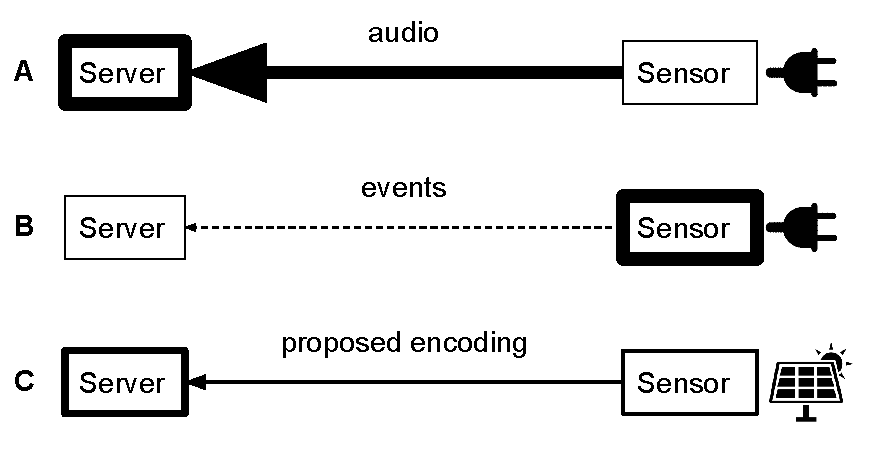
\includegraphics[width=0.5\textwidth]{figures/censeCoder}
\caption{Alternative implementations of the sensor grid approach for the monitoring of the acoustic environment. In A) the raw audio is transmitted, in B) only the detected events, and in C) a compressed spectral representation. Thickness of arrows indicates bandwidth and thickness of boxes indicates the level of computation or storage required.}
\label{fig:codingScheme}
\end{figure}


\section{Background} \label{sec:background}


The main contribution of this paper is to present an acoustic data encoding scheme that allow both acoustic monitoring and sound event recognition in urban sound environment. Here we briefly review state-of-the-art methods in both subjects in order to better motivate our design choices.

\subsection{Acoustic monitoring}

The considered sensor network primarily aims at monitoring urban sound environment, that is, continuously assessing their content and impact on the population. In the literature, this is typically performed by measuring energetic acoustic indicators such as the equivalent sound pressure level $L_{eq}$ in dB SPL or its A-weighted equivalent $L_{Aeq}$ in dBA. However, while these indicators have proven to correlate well with perceptual evaluations for negative impact sound environments \cite{gozalo2015}, they are not sufficient to fully describe urban sound environments \cite{rychtarikova2013}. Many other variables can be derived to better account for previously implicit properties \cite{can2016} including percentile values or time dynamics. Studies have been conducted to select relevant subsets of descriptors in sound environment characterization \cite{can2015, brocolini2013, nilsson2007}. The mentionned $L_{eq}$ features are measured at periods of 0.125~ms or 1~s, respectively termed as "fast" and "slow" as a convention.

Most measured or derived indicators describe the global urban acoustic environment and lack information on its composition. Sound sources recognition enables a more comprehensive understanding of the properties of the acoustic environment. For instance, a bird song and traffic noise with the same energy are perceived very differently. The analysis of sources within a sound environment is generally linked with spectral content \cite{ishiyama2000} and high temporal measurement resolutions. Other indicators can correlate with specific sound environment content \cite{aumond2017} but do not achieve the level of performances of a good source detection scheme in characterizing acoustic environments.



\subsection{Event detection}

As discussed in the previous section, the recognition and the estimation of the level of contribution of sources of interest is of importance to fully model the studied acoustic environments, see for example \cite{alsina2016design, app7020146, gloaguen2016estimating}. As far as the encoding scheme is concerned, it is thus important that the encoded data allows us to compute the above cited indicators but also to detect the different sound sources with state of the art methods.

The recognition of sources of interest from audio streams has been the subject of extensive research in the past on speech \cite{anusuya2009}, music \cite{tzanetakis2002}, and lately more complex scenes in which the current work falls. Studied classification methods are diverse, ranging from time-dependant modeling with hidden markov models \cite{ntalampiras2014} to "bag-of-frames" approaches \cite{aucouturier2007, foggia2015}. Common architectures include learning-based classifiers such as support vector machines \cite{kumar2016}, Gaussian mixture models \cite{radhakrishnan2005} or neural networks \cite{salamon2017, piczak2015}. However, the selection of relevant features is still an open debate. The most used are certainly spectral \cite{khunarsal2013} or cepstral \cite{couvreur2004} representations of the signal. Among them, Mel spectrograms and their cepstral-domain derivation, the Mel-frequency cepstrum coefficients (MFCC), are the most recurrent. These representations effectively model the human cochlear response to sounds by grouping frequency components around critical bands in a logarithmic scale. While parameters are empirical and vary in the literature, a reference implementation includes 23.2~ms analysis and a 40 Mel bands resolution. The resulting representations are generally more precise in time and frequency than in acoustic monitoring applications because it is a primordial factor for classification whereas acoustic indicators must be computed more accurately.

They may also be exploited together with features computed in other domains to better model signal properties. For instance, \cite{cai2006} adds spectral features related to harmonicity and salient frequencies, and \cite{chu2009} uses a matching pursuit (MP) algorithm to deduce time-domain features. Another promising solution is feature engineering via unsupervised learning, which \cite{salamon2015-2} implements with a clustering technique. Alternative data representations such as the scattering transform \cite{bauge2013} show good results in environmental sound classification tasks \cite{salamon2015}.\\
A more detailed review of used methods is available in \cite{chachada2013}.

\section{Encoding scheme} \label{sec:coder}

We thus need to provide data that allows both the computation of previously described indicators and the recognition of sound events.
To do so, we propose to consider the calculation of spectral energetic indicators such as the 31 third-octave bands within the human audition range 20~Hz - 20~kHz.\\ Slow or fast third-octave bands measurement appears suitable for this work's purpose: in addition to being a relevant descriptor \cite{torija2013} for urban sound environment assessment, it allows for the computation of most cited indicators while representing reasonably small, fixed amounts of data to be transmitted. It additionnaly contains spectral information that can be used for source recognition tasks as it is close to the Mel spectral representation, being just another filterbank transform with logarithmic frequency scaling.

A common way to implement third-octave analysis is to first design the highest octave three filters, and use them on progressively time-decimated versions of the input signal \cite{davis1986}. Antoni et al. \cite{antoni2010} presents an alternative analysis method based on direct frequency weighting, which yields a lower computational complexity as opposed to time filtering. The weights matrix design procedure complies with both ANSI S1.1-1986 \cite{citeulike:9580295} and IEC 61260-1:2014 \cite{iec-norm} standards. It also meet the partition of unity principle over all frequency bins in the relevant range. Resulting filters for different parameter $l$ values are compared with Couvreur's implementation \cite{couvreur} of the time-domain filtering, as shown in Figure~\ref{fig:freq_filt}. The major difference is that gains at cutoff frequencies are fixed at the optimal -3dB value by design.\\

\begin{figure}[htbp]
	\centering
		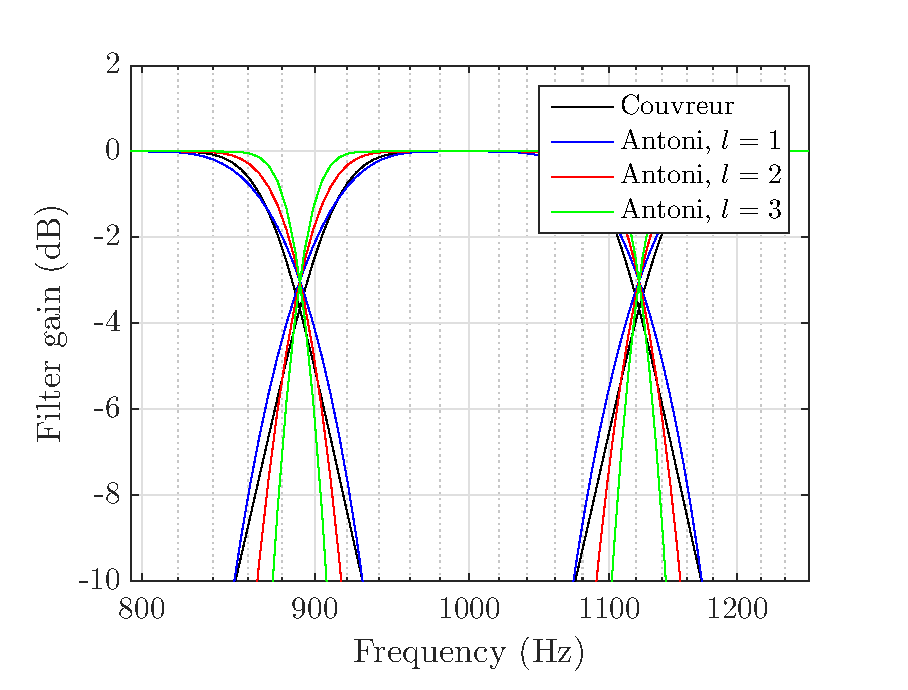
\includegraphics[width=0.8\textwidth]{figures/tob_imp.eps}
	\caption{Comparison of Couvreur's and Antoni's implementations of third-octave filters. Frequency-weighting allows for arbitrary transfer functions and thus more accurate gains as standards impose.}
	\label{fig:freq_filt}
\end{figure}

The first step is to represent the signal in the frequency domain using a short-term Fourier transform (STFT). The continuously sampled audio is segmented into either 125~ms or 1~s frames to provide "fast" or "slow" acoustic measurements. The data is zero-padded to the next power of two to improve computational efficiency. The other parameters such as windowing functions and frame overlap are dependant on the specific constraints, and discussed in section \ref{sec:protocol}. The phase is discarded as it is not meaningful for third-octave analysis. Similarly, negative frequency components contain the same information as positive ones because the input signal is real. We then compute third-octave bands from the squared spectral magnitude by matrix multiplication with the frequency weights proposed in \cite{antoni2010} for $l = 2$\footnote{When implementing said method, we found that squaring the $\phi_l(p), l \geq 1$ intermediate function (p. 887) was the correct approach to meet cutoff frequencies requirements, and we believe this was the author's original intention.}. We include analysis for bands $i$ from -17 to 13, ie. center frequencies $f_i$ ranging from $20~Hz$ to $20~kHz$ with $f_0 = 1~kHz$. The representation is thus composed of 31 values.


\subsection{Data Encoding}

A Huffman coding scheme \cite{huffman1952} is an efficient method to further reduce data rate while keeping the underlying information. At this point of the processing chain, the data takes the form of a spectrogram with amplitude values represented on an arbitrary data type. It is therefore assimilable to a discrete distribution. By defining symbols as the possible values taken by the data, a discrete probability density function (PDF) can be expressed and estimated. The Shannon entropy then specifies the minimum average achievable output data rate for this given distribution, or average information content. The Huffman algorithm is an entropy coding scheme, as it uses the PDF to assign a code to each symbol so that the average output rate is the closest to the entropy. The resulting mapping function is called a Huffman dictionary.

The efficiency of the coding step thus directly depends on the entropy of the transmitted data. It is defined as $H = -\sum\limits_i p_ilog_n(p_i)$, where $p_i$ is the probability of appearance of a given symbol $i$ and $n$ the numerical base in which the output code is represented. A lower entropy can be obtained with two factors. First, the dictionary size \textit{i.e.} the number of symbols must be kept low. This implies performing a quantization on the data resulting in a loss of precision. Second, the data distribution itself is important. Entropy decreases when very few symbols have a very high probability of appearance and is maximum for a uniform distribution.

Considering an estimated PDF for our data as shown in Figure~\ref{fig:pdf} (top-left), immediately applying a linear quantization is clearly suboptimal, as the data mostly consists of very low values and a direct quantization results in most of the information being lost. We therefore flatten the PDF by taking the logarithm of the representation (top-right). This allows to better use the available range of symbols. A linear quantization is then applied with $2^{q-1}-1$ output values to obtain Figure~\ref{fig:pdf} (bottom-left). Finally, we use a $\Delta$-encoding algorithm along the time dimension to reduce redundancies between consecutive frames. This effectively concentrates higher probabilities on symbols around zero (Figure~\ref{fig:pdf} bottom-right), yielding a higher amount of symbols at $2^q-1$ but nevertheless a smaller entropy. In the example shown here, the entropy before $\Delta$-compression is $H_{log} = 6.24~sh$ which is reduced to $H_{\Delta} = 3.54~sh$.

Huffman encoding is then computed with either a frame-specific symbol-code dictionary or a fixed dictionary generated using a learning dataset. A comparison of both methods is shown in Figure~\ref{fig:dict_comp}. For most short texture frame durations, the local Huffman algorithm is found to be much faster. In fact, the encoding computational complexity is a function of the number of dictionary elements. A frame-specific dictionnary only contains the symbols found in a given data packet, while a fixed dictionnary must contain every possible symbol as it does not depend on the present data. The output bitrate is found to be close for both methods, as sending an optimal local dictionnary balances the suboptimality of globally generated symbol-code pairs.\\

\begin{figure}[htbp]
	\centering
		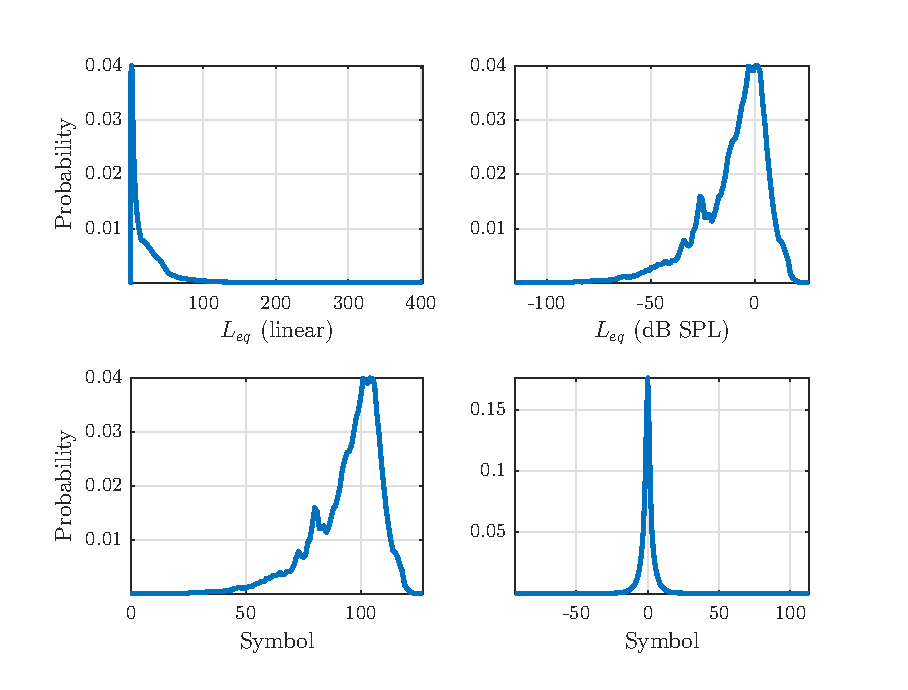
\includegraphics[width=0.8\textwidth]{figures/pdf.eps}
	\caption{Example of estimated probability density functions of the data throughout the encoding step. Unchanged output of the representation step (top-left), concentrated towards very low values. PDF "flattening" effect induced by logarithm application (top-right). Here values are mapped to the range $[0, 2^7-1] (q=8)$ and rounded to perform quantization (bottom-left). Output of the $\Delta$ compression (bottom-right), with desirable probabilities as the input to a Huffman algorithm.}
	\label{fig:pdf}
\end{figure}

\begin{figure}[htbp]
	\centering
		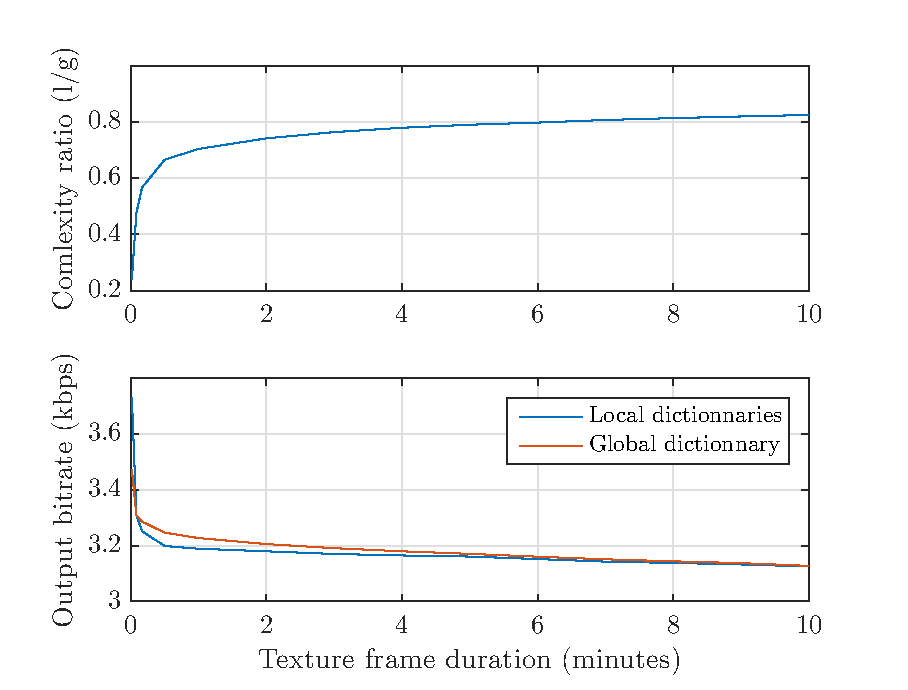
\includegraphics[width=0.8\textwidth]{figures/dict_comp.eps}
	\caption{Performance comparison of locally and globally generated Huffman dictionaries. (top) The mean execution time ratio favors the use of frame-specific dictionaries for tested texture frame lengths. (bottom) The mean output bitrate is close for both algorithms, showing that the necessity of sending symbol-code pairs mostly compensates for their optimality.}
	\label{fig:dict_comp}
\end{figure}

The decoding process is quite straightforward, as both Huffman and $\Delta$ compressions are lossless and directly invertible. The entire coder scheme is summarized in Figure~\ref{fig:scheme}.

\begin{figure*}[htbp]
	\centering
		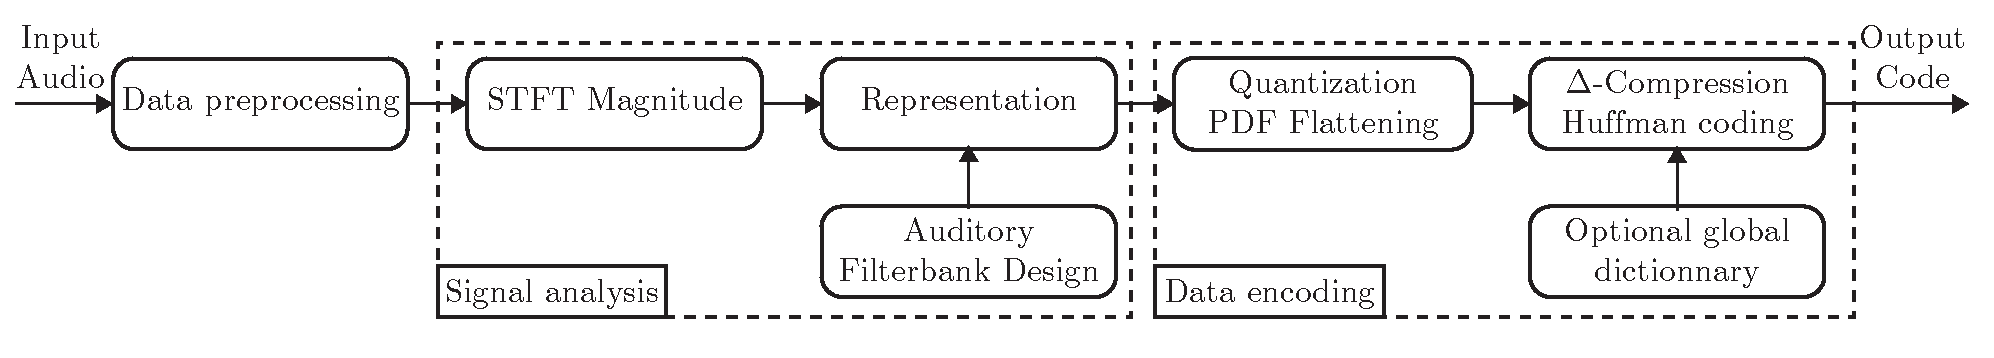
\includegraphics[width=.9\textwidth]{figures/scheme.pdf}
	\caption{Overview of the coder process.}
	\label{fig:scheme}
\end{figure*}

\section{Validation protocol} \label{sec:protocol}

A set of metrics is computed to assess the efficiency of the proposed coder scheme and to determine the impact of the degrees of freedom given by the parameters of the proposed algorithm. Those parameters are as follow: 1) the desired word size prior to Huffman encoding, set by quantization for both signal representation choices, 2) the number of considered bands, and 3) the STFT parameters including frame duration, overlap and windowing function usage.

\subsection{Efficiency}

The coder's output bitrate as well as measurement error is computed for both data representations. This metric is composed of band analysis error and the additional loss yielded by quantization before the encoding process.


To evaluate the analysis error, we consider the Matlab \textit{ita\_toolbox} implementation \cite{itatoolbox2017} as a reference. We study both "fast" computation with 125~ms windows and "slow" 1~s analysis to assess the impact of time integration. Third-octave bands are computed using the proposed method as well as the \textit{ita\_toolbox} in the same experimental conditions, then averaged over time and compared to the toolbox's measurements on longer extracts. In all experiments the sound dataset is the same and is composed of 2~s extracts. The experiment is run for white noise as well as urban environmental recordings. As the analysis frames are of short duration, poor frequency resolution and spectral leakage are expected, particularly in the lower frequencies bands. For this reason we evaluate the effect of the use of windowing functions on each band measurement error in order to mitigate this loss of precision. To provide relevant statistics, these quantities are estimated with data from the 4500 audio recordings of the UrbanSound8k dataset \cite{salamon2014} described in the next section and 4500 \textit{iid.} noise sequences.

\subsection{Event recognition}

In order to ensure that the proposed scheme allows the recognition of events using state of the art methods, we consider the results achieved by several recognition systems on the UrbanSound8k dataset\cite{salamon2014}. It features about 9 hours of urban environmental sounds recordings separated in 8732 wave files ranging from 1 to 4 seconds each. The recordings are labeled in 10 classes (air conditioner, car horn, children playing, dog bark, drilling, engine idling, gun shot, jackhammer, siren, street music), and distributed in 10 independent folds. A method and baseline results are also provided for the classification task. It is used in all the following experiments with the exception of intelligibility computation for which a small dataset of high-quality voice recordings is preferred. Audio files are resampled at 44.1~kHz, normalized and a single channel is considered.

Mel spectrograms are computed with the \textit{rastamat} library \cite{ellis2005} to assess the relative performance of third-octave bands. STFT analysis frames are obtained by applying a Hann window on 23.2~ms of signal with 50\% (11.6~ms) overlap to allow for efficient phase recovery in further tests.

We evaluate the global loss of information induced by the coder by implementing the four classification models proposed in \cite{salamon2014}: a support vector machine with a radial basis function kernel, a random forest classifier with 500 trees, a decision tree and a k-nearest neighbors classifier with $k = 5$. Values for the SVM parameter $C$ and RBF kernel variance $\sigma^2$ are found with a grid search. We optionally apply a discrete cosine transform to the critical band signal representation to obtain cepstra, known as Mel Frequency Cepstrum Coefficients or MFCC in the case of Mel spectrograms. The 25 first coefficients are conserved, and summarized along time with the mean, variance, skewness, kurtosis, minimum, maximum, median, derivative mean and variance, second order derivative mean and variance operators. The feature vector is thus comprised of 275 values to reproduce available results and compare with the data produced by the proposed coding scheme. Models are trained for each setup using the 10-fold cross validation method provided by the authors of \cite{salamon2014}, that is, every combination of testing one fold on models trained with the other nine.

\subsection{Inintelligibility} \label{sec:inintelligibility}

It is important that the proposed scheme ensures a high level of recognition of acoustic events but, as the data is transmitted over the network and potentially stored, the level of intelligibility of potenital speech utterances present in the decoded stream should be as low as possible. Thus, intelligibility in decoded and reconstructed audio is also an important concern of this study.

The use of an audio recording as an evidence is considered by the forensic phonetics \cite{baldwin1990forensic} field. The readers shall be aware that even recorded with a good quality, such recording remains a weak biometrical indicator \cite{boe2000forensic}. Still, even if the identity of the speaker cannot be asserted, one can attempt to transcribe the spoken utterances. As such, we believe that it is important to demonstrate that the proposed encoding scheme do not allow such thing.

In order to decrease the intelligibility, several approaches can be considered. First,  a speech versus non speech detector can be implemented on the sensor. If some speech is detected, the data is not transmitted. This approach is however prone to failure of the detector and will lead to unavailability of data during speech time periods which might compromise the relevance of some indicators.

Second, as the speech is mostly concentrated at a given frequency region, a band-pass filter from 1 kHz to $~$4-5 kHz could be considered in order to remove the formant information \cite{kent1992acoustic}. However, as some frequency bands are no longer available, the computation of standard acoustic indicators is no longer possible.

A third approach is to wisely choose the frame rate. Since a phoneme is about 100ms to 200ms long \cite{kuwabara1996acoustic} \cite{rosen1992temporal}, a frame rate lower than 4 Hz should therefore dramatically reduce intelligibility.

Thus, the impact of the frame rate parameter of the proposed encoding scheme on intelligibility is evaluated. To do so, a perceptual test is conducted. For the evaluation, a dataset of clean speech recordings made of 9 french sentences enunciated by 3 male and 3 female speakers. The recorded sentences are encoded using the proposed approach with 4 analysis frame rate parameters of respectively 50~Hz, 16~Hz, 8~Hz and 4~Hz. As a result, 216 audio excerpts with a duration of about 2 seconds are tested in total.

For the perceptual test, each subject is presented with sentences and asked both to transcribe the utterances and rate the global intelligibility from 1 (not intelligible) to 5 (intelligible). Due to the low number of sentences, each sentence is tested twice for the same subject but under different encoding setting and speaker identity, resulting in each subject evaluating 18 extracts. 12 subjects of age ranging from 17 to 60 which reported normal hearing participated to the listening test. The test was conducted using a Matlab interface displayed with a desktop computer and audio was played through \textit{Beyerdynamics DT 770} headphones. The output level was set by the experimenter at the same level for all subjects.

This test requires an estimate of the time-domain signal. To do so, a linearly-scaled spectrogram from the band-focused representations is estimated. This estimation can be achieved by multiplying the spectral representation by the scaled transpose of the forward transformation matrix. A loss of resolution increasing with frequency is induced due to the shape of the transformation, as illustrated by Figure~\ref{fig:freq}. Signal phase is then approximated by either white noise spectrogram scaling or the Griffin \& Lim algorithm \cite{griffin1984} in hte case of overlapping frames. The signal is then retrieved using concatenation or overlap-add depending on the overlap setting. When using overlap to compute third-octave bands, one can also avoid framing effects produced by rectangular windowing by convoluting the signal with another windowing function prior to inverse-STFT computation.

\begin{figure}[htbp]
	\centering
		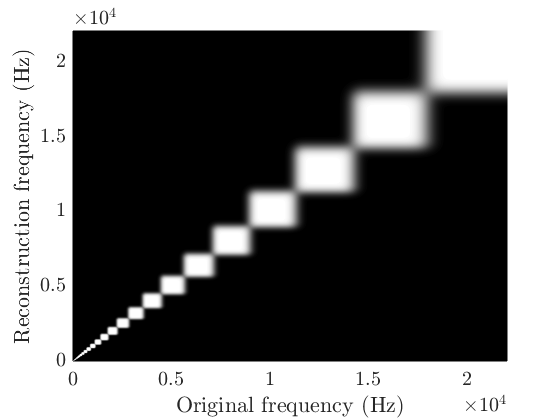
\includegraphics[width=0.5\textwidth]{figures/freq.png}
	\caption{Third-octave bands analysis and approximate inverse transformation effects on energy location. This process yields an important and heterogeneous loss in resolution, particularly at higher frequency points.}
	\label{fig:freq}
\end{figure}



\section{Results} \label{sec:results}

\subsection{Coder efficiency}

The main indicator of performance is the bitrate obtained at the output of the coder. The three varying factors studied are the data word size $q$, the number of bands and the effect of reducing time-resolution by averaging analysis frames. Figure~\ref{fig:bitrate_q} shows estimations of the output bitrate for different values of $q$. To match third-octave bands computation principle where a 125~ms analysis is mandatory, Mel frames are averaged over time. Because we use the most common parameters, namely 23.2~ms window with 50\% overlap, the closest achievable rate considering simple averaging is 7.74 frames per second. Third-octave representation on 31 bands yields an overall higher size than their Mel equivalent, here estimated for 30 bands. It however compares with the 40-Mel bands representation which is the most used features in literature. This higher bitrate is likely due to the distribution observed by the data prior to Huffman encoding.

\begin{figure}[htbp]
	\centering
		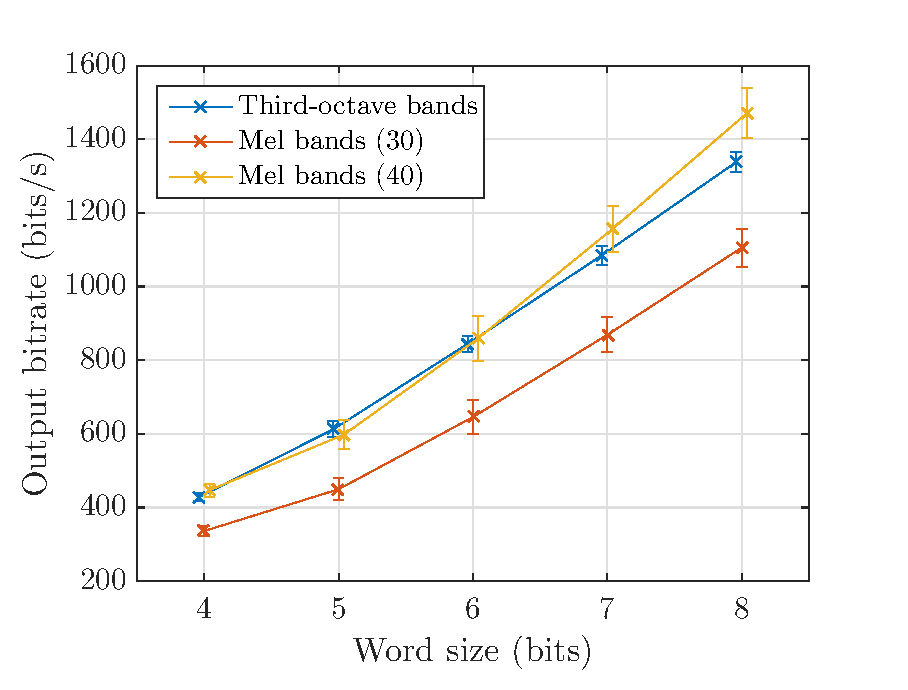
\includegraphics[width=0.8\textwidth]{figures/bitrate_qall.eps}
	\caption{Coder output bitrate as a function of quantization for third-octave and Mel bands with 8 frames per second.}
	\label{fig:bitrate_q}
\end{figure}

A second set of parameters influences directly the time-frequency resolution of the analysis. By choosing a frame rate and number of bands, one can effectively control the size of the periodically transmitted data. We evaluate the bitrate for 10 to 40 Mel bands and a frame rate from 2 to 10 per second, with fixed $q = 8$. Results are shown in Figure~\ref{fig:bitrate_mel_avg}. As expected, the bitrate for a given word size $q$ can be modeled as a linear function of the representation dimensions for one second of analysis. Small variations are induced by data distributions on a per-frame level and their impact on the Huffman algorithm.

\begin{figure}[htbp]
	\centering
		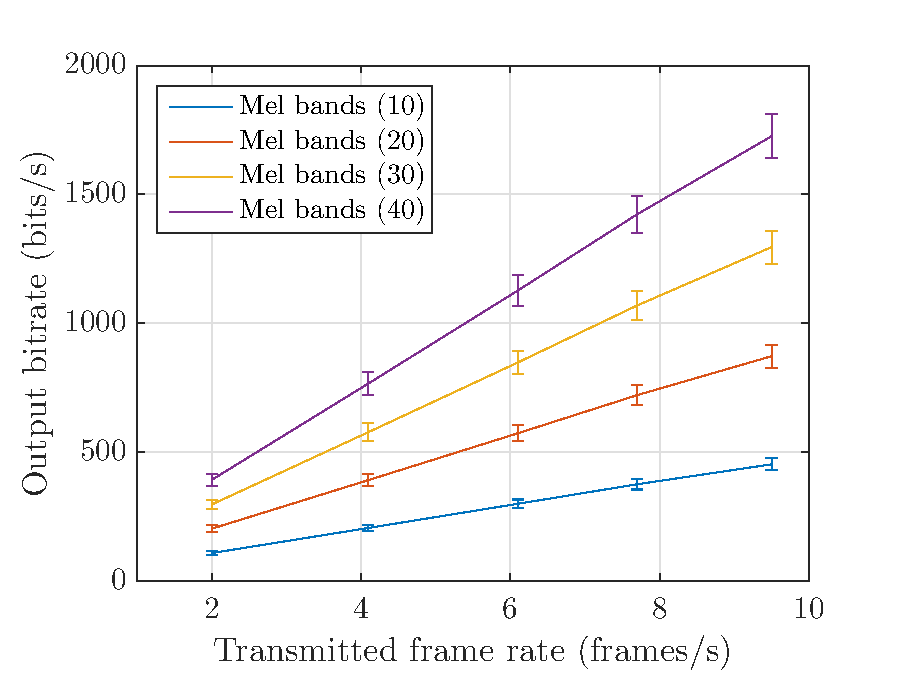
\includegraphics[width=0.5\textwidth]{figures/bitrate_mel_avg.eps}
	\caption{Impact of representation resolution on the encoded data bitrate.}
	\label{fig:bitrate_mel_avg}
\end{figure}

This experiment aims at an initial assessment of potential tradeoffs between bitrate and preservation of valuable information which will be further discussed in Section \ref{sec:eventRec}.\\

The measurement error is now computed for third-octave bands. Results are displayed in Figure~\ref{fig:errormn} for white noise extracts and in Figure~\ref{fig:errormu} for environmental sounds. Only full-octave bands are shown for the sake of visibility. When computing the slow analysis, we find that applying overlap attenuated the error. This is not observed for fast analysis where the error is similar or higher with the use of overlapping frames.

As can be expected when performing a short time analysis, high errors appear in low frequency bands where precision is poor. The slow analysis yields better estimations as it provides a globally better resolution and thus also reduces the impact of spectral leakage effects in this region. When considering white noise the error is low on the whole spectrum. Its mean over the testing samples is close to zero and its standard deviation increases in low frequencies, confirming the above-mentioned considerations. This effectiveness does not translate well to environmental sound analysis, most likely mainly due to the sound level disparities absent in the former case but omnipresent in the latter. Spectral leakage induces a correlation between close frequency components. In lower frequencies, large differences between adjacent frequency bins can thus cause important errors on third-octave bands computations. This issue is however not specific to Fourier transform based schemes as it is also encountered with a time domain filtering approach.

To mitigate this phenomenon, the choice of the window function shall be studied further. For a fast analysis with no overlap, the rectangular window seems a reasonable choice at first because of its energy conservation qualities. While it yields the lowest error in high frequency bands, its high spectral leakage effect makes it unprecise for lower frequency regions. Non-flat windows better account for this issue but require assuming that the signal is stationary in a given frame. The use of overlap then results in better estimates at the cost of an increased data size. For slow measurements, considering the rectangular window impact is less harmful to band analysis due to an increased frequency resolution.

The comparison of the error achieved by the proposed scheme to that of third-octave bands estimated by a reference time-filtering algorithm is now considered. It results in important similarities. For fast measurements and a rectangular window (Figure~\ref{fig:errormu}a), a student t-test ($p<0.05$) shows that the errors are not significantly different between 125~Hz and 12~kHz bands. For the first bands, the two methods yield different error distributions but of similar importance. Using a Hann window function results in lower error in low frequencies but adds a bias to the previously accurate band measurements. Again comparing the two computation methods shows a significant difference in the bands below 100~Hz only. A slow analysis results in statistically equivalent errors between the two methods apart from the very low frequencies: $p = 0.011$ with the rectangular window (Figure~\ref{fig:errormu}c), $p = 0.003$ at 20~Hz and $p = 0.021$ at 25~Hz for the Hann window and 66\% overlap (Figure~\ref{fig:errormu}d).\\

\begin{figure}[h!]
    \centering
    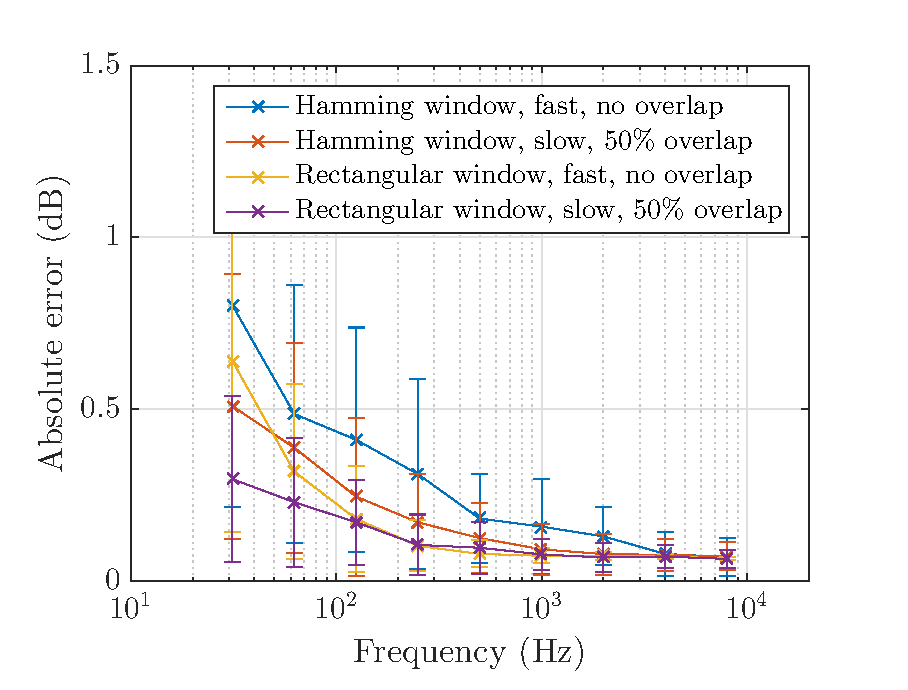
\includegraphics[width=0.5\textwidth]{figures/err_m_n.eps}
    \caption{Measurement error of third-octave bands over two-seconds white noise extracts, with rectangular window and no overlap. The analysis of short frames has an effect on energy estimation at low frequencies that is of lower importance as the frequency resolution increases.\label{fig:errormn}}
\end{figure}

\begin{figure*}[h!]
    \centering
    \begin{subfigure}[h]{0.45\textwidth}
        \centering
        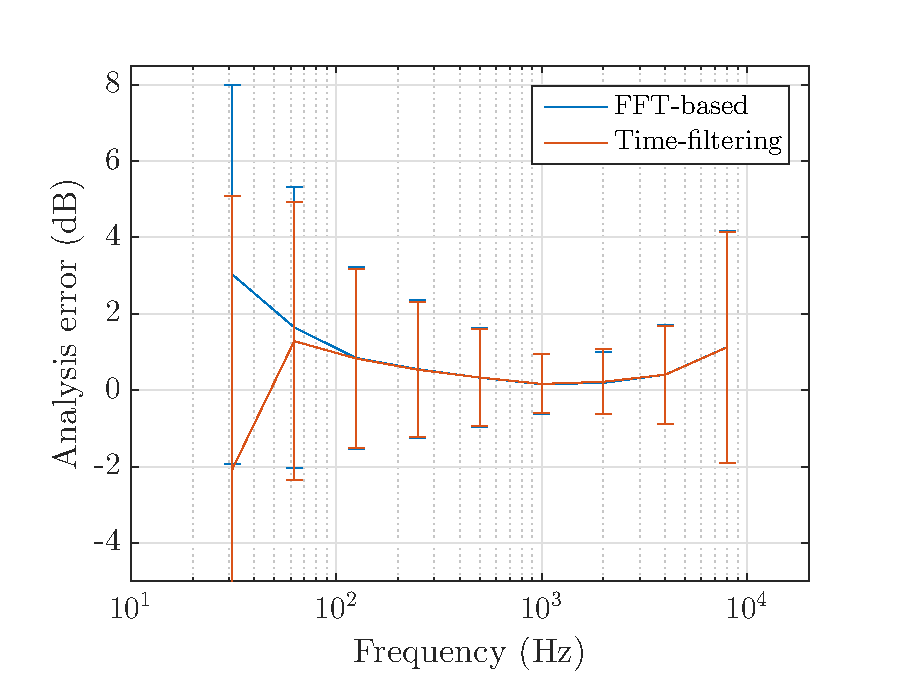
\includegraphics[width=1\textwidth]{figures/err_m_u_f_r.eps}
        \caption{Fast analysis, rectangular window, no overlap}
    \end{subfigure}
    \hfill
    \begin{subfigure}[h]{0.45\textwidth}
        \centering
        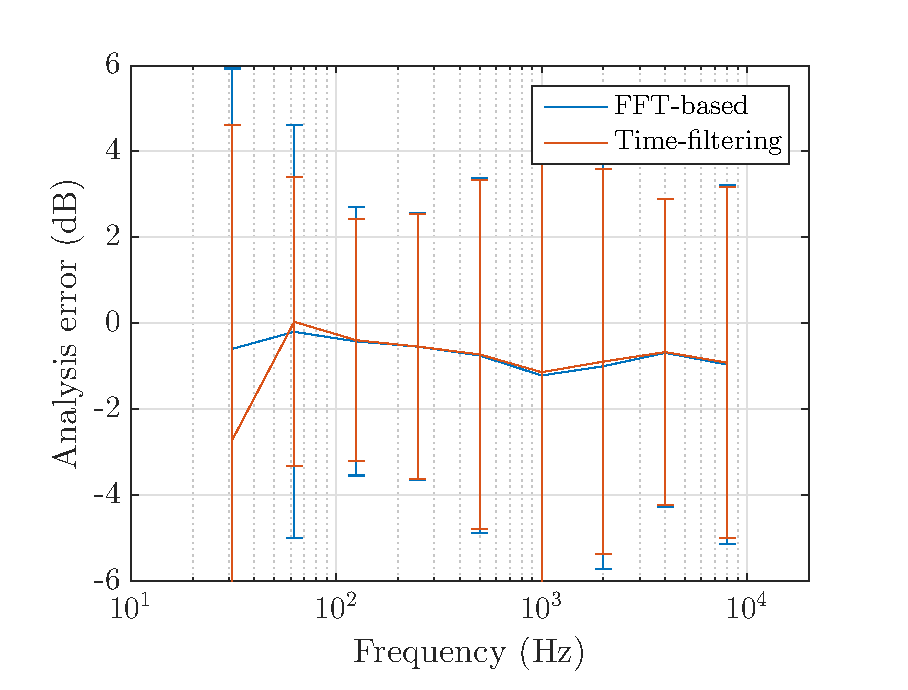
\includegraphics[width=1\textwidth]{figures/err_m_u_f_h.eps}
        \caption{Fast analysis, Hann window, 66\% overlap}
    \end{subfigure}
	\begin{subfigure}[h]{0.45\textwidth}
        \centering
        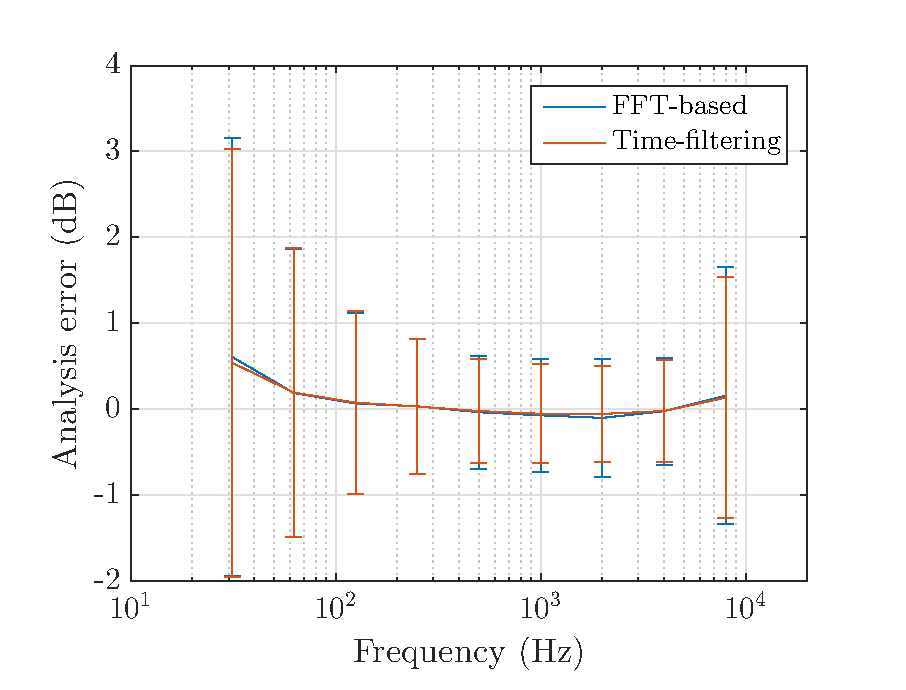
\includegraphics[width=1\textwidth]{figures/err_m_u_s_r.eps}
        \caption{Slow analysis, rectangular window, 50\% overlap}
    \end{subfigure}
    \hfill
    \begin{subfigure}[h]{0.45\textwidth}
        \centering
        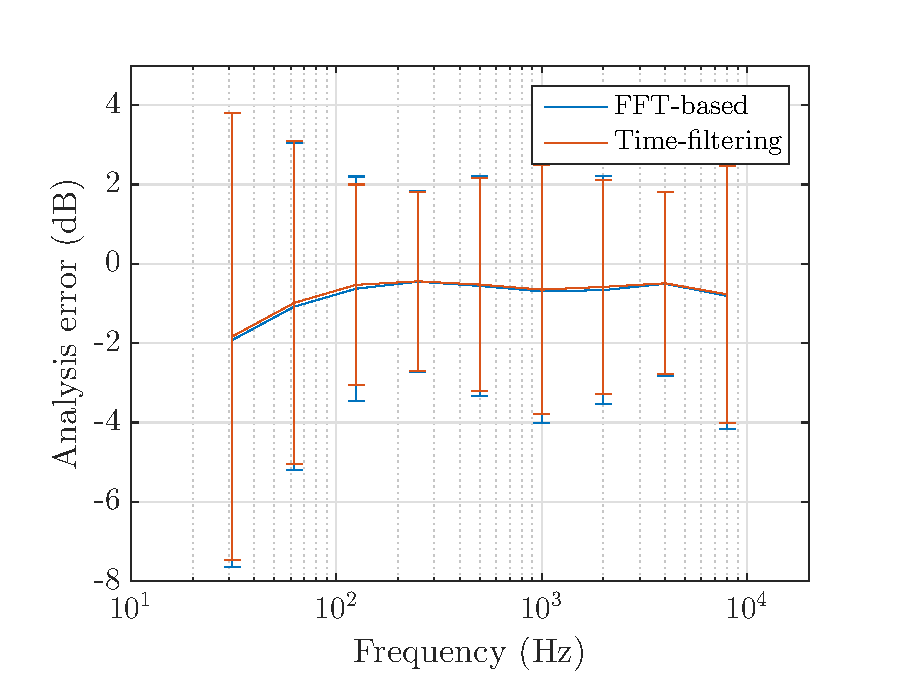
\includegraphics[width=1\textwidth]{figures/err_m_u_s_h.eps}
        \caption{Slow analysis, Hann window, 66\% overlap}
    \end{subfigure}
    \caption{Measurement error of third-octave bands over two-seconds environmental sounds recordings (US8k dataset). For most settings the FFT-based method yields similar errors to the time-domain filtering reference. \label{fig:errormu}}
\end{figure*}


We also examine the additional error caused by the encoding steps after obtaining the desired data representation. The only lossy operation applied is quantization, which is defined by an output word size $q$ in bits. However, it corresponds to the word size \textit{after} $\Delta$-compression, meaning that the data is in fact quantized on $2^{q-1}$ values. Since these measurements are already expressed in dB, the error $\varepsilon$ is:
\begin{equation*}
	\varepsilon = |x_q-x|
\end{equation*}
where $x_q$ and $x$ are the quantized and clean representations repectively. $x_q$ is given by:
\begin{equation*}
x_q(n) = \frac{\Delta_x}{2^{q-1}-1}\textrm{round}\left(\frac{(2^{q-1}-1)x(n)}{\Delta_x}\right), x\in \left[0, \Delta_x\right]
\end{equation*}
Figure~\ref{fig:error_q} shows an estimation of $\varepsilon$ as a function of $q$ for third-octave and Mel bands. In both cases, the mean and standard deviation seem to decrease by a factor of 2 as $q$ increases. To better understand this phenomenon, let us model $x$ as a uniform distribution such as $x\sim \textit{U}\{0, \Delta_x\}$. While this is not exact it matches our objective when using a logarithm to flatten given PDFs. The error $\varepsilon$ will follow a uniform distribution $U\sim \{0, \frac{\Delta_x}{2\times (2^{q-1}-1)}\}$. Therefore, the mean and standard deviation are:
\[
\begin{cases}
	\mu_\epsilon = \frac{\Delta_x}{4\times (2^{q-1}-1)}\\
	\sigma_\epsilon = \frac{1}{12}\frac{\Delta_x}{2\times (2^{q-1}-1)}
\end{cases}
\]
justifying the decaying ratio as $q$ increases. In practice, we assume that $\varepsilon = f(\Delta_x, \frac{1}{2^{q-1}-1})$ with the heterogeneity of the data's PDF inducing small variations.

\begin{figure}[htbp]
	\centering
		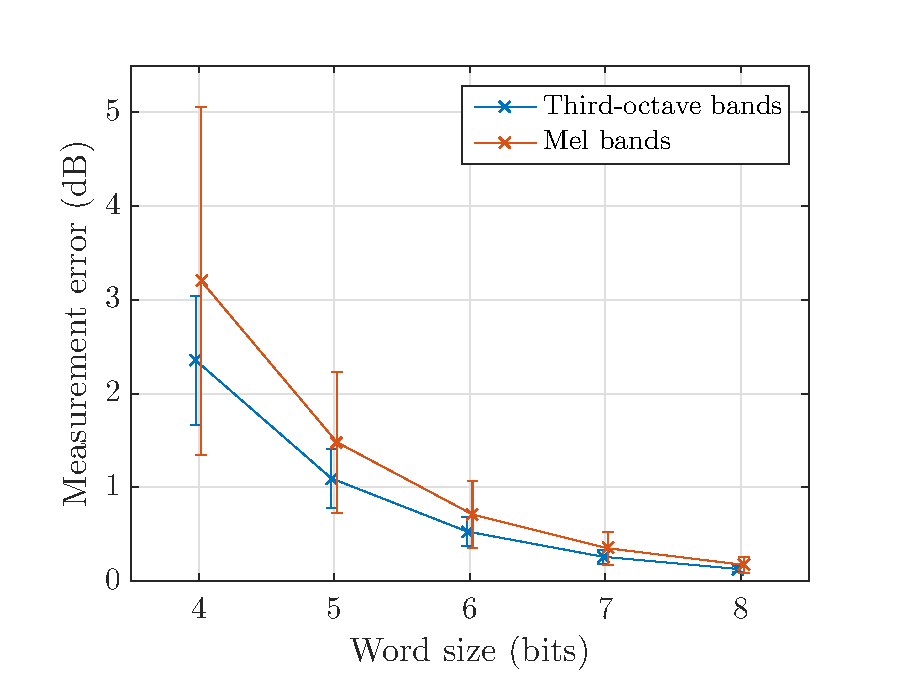
\includegraphics[width=0.5\textwidth]{figures/error_qall.eps}
	\caption{Measurement error induced by encoding for different quantization resolutions.}
	\label{fig:error_q}
\end{figure}


As $\Delta_x$ is sampled for each analysis frame in our implementation, the error has the same statistics across all bands. It is to be added to the measurement error discussed in the same section before comparing to the values specified in the IEC 61672-1:2013 \cite{iec-norm2} standard on class 1 and 2 sound level meters.

\subsection{Event recognition} \label{sec:eventRec}

The same set of parameters as in bitrate evaluation is used to study the impact of their tuning to the sound event recognition performance. We thus aim at finding ways to further reduce the encoded data size without strongly affecting recognition performance. Results of the four presented classification methods are provided for the sake of completeness.\\

First, we observe the impact of quantization on classification accuracy. The models are trained on the most complete implemented representation, ie. 40 Mel bands, 23.2~ms, 50\% overlap and no time averaging (85 frames per second). Figure~\ref{fig:class_mel_q} shows that this process yields equivalent accuracy for higher resolutions.\\

\begin{figure}[htbp]
	\centering
		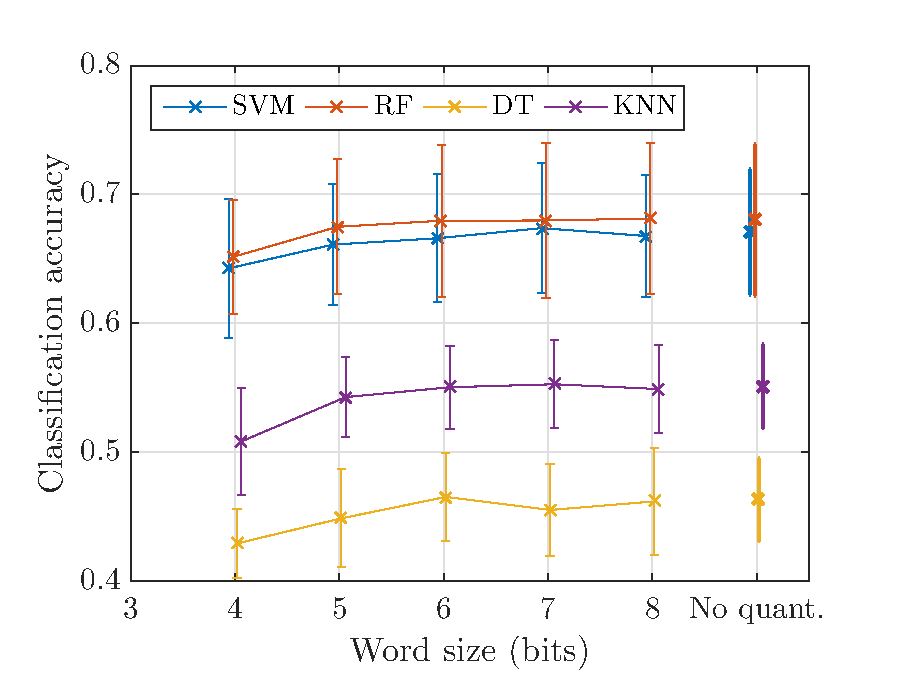
\includegraphics[width=0.5\textwidth]{figures/class_mel_q.eps}
	\caption{Classification accuracy as a function of word size before encoding. The baseline on the right is computed without quantizing the representation.}
	\label{fig:class_mel_q}
\end{figure}

The effect of changing the time-frequency resolution of the representation is presented in Table~\ref{T2}. Similarly to baseline results, the random forest and SVM classifiers are the higher performing systems at $0.69\pm 0.06$ and $0.68\pm 0.04$ respectively. However, we find that given our setup, reducing the number of analysis bands up to a given level most often does not induce a strong drop of performance. The performance of the decision tree classifier is a good example of this behavior, with best performances for 10 Mel bands only and a 4\% lower accuracy for 40. Even if the difference is small, all other models perform best with 30 or 40 Mel bands as a representation. Time decimation can also be considered, as the original representation can be averaged and consistently yield a good classification accuracy. The loss of information can be considered negligible for FPS values as low as 20 or 10 depending on the method. Even below, classification accuracy only drops by one or a few percents. This means that we can effectively divide the data size by a factor of at most 10 without strongly affecting sound event recognition performance. It also provides us with a preliminary confirmation of the possibility for "fast"-sampled third-octave bands cepstra to match  MFCC performances.\\

\begin{table*}[h]
\centering
\caption{Classification accuracy in percentage for different classifiers: SVMs (a), Random Forests (b), Decision Trees (c), and Nearest Neigbors (d) with respect to varying representation resolutions. Numbers in red indicate best performance and numbers in bold indicate that no statisticaly significant difference is found when comparing to the best performing setting ($p<.05$).}
\label{T2}
(a)\\
\begin{tabular}{ll|c|c|c|c|c|c|c|}
\cline{3-9}
\multicolumn{2}{c}{\multirow{2}{*}{SVM}} & \multicolumn{7}{|c|}{Frames per second}\\ \cline{3-9}
 & & 2 & 4 (4.1) & 6 (6.1) & 8 (7.7) & 10 (9.5) & 20 (21) & 85 \\ \cline{1-9}
\multicolumn{1}{|c}{\multirow{4}{*}{Mel bands}}
 & \multicolumn{1}{|c|}{10} & 55$\pm$3 & 60$\pm$3 & 61$\pm$4 & 62$\pm$3 & 62$\pm$4 & \textbf{63$\pm$6} & \textbf{65$\pm$6} \\ \cline{2-9}
\multicolumn{1}{|c}{}
 & \multicolumn{1}{|c|}{20} & 58$\pm$4 & 62$\pm$4 & 63$\pm$4 & 64$\pm$4 & 63$\pm$4 & \textbf{65$\pm$5} & \textbf{67$\pm$6} \\ \cline{2-9}
\multicolumn{1}{|c}{}
 & \multicolumn{1}{|c|}{30} & 60$\pm$3 & 64$\pm$4 & 64$\pm$4 & \textbf{65$\pm$4} & \textbf{65$\pm$3} & \textbf{67$\pm$4} & \textbf{\textcolor{red}{68$\pm$4}} \\ \cline{2-9}
\multicolumn{1}{|c}{}
 & \multicolumn{1}{|c|}{40} & 60$\pm$3 & 63$\pm$4 & \textbf{64$\pm$4} & 64$\pm$4 & \textbf{64$\pm$4} & \textbf{66$\pm$4} & \textbf{68$\pm$5} \\ \cline{1-9}
\end{tabular}
\\(b)\\
\begin{tabular}{ll|c|c|c|c|c|c|c|}
\cline{3-9}
\multicolumn{2}{c}{\multirow{2}{*}{RF-500}} & \multicolumn{7}{|c|}{Frames per second}\\ \cline{3-9}
 & & 2 & 4 (4.1) & 6 (6.1) & 8 (7.7) & 10 (9.5) & 20 (21) & 85 \\ \cline{1-9}
\multicolumn{1}{|c}{\multirow{4}{*}{Mel bands}}
 & \multicolumn{1}{|c|}{10} & 60$\pm$3 & 62$\pm$3 & 62$\pm$3 & 63$\pm$3 & 63$\pm$3 & \textbf{65$\pm$4} & \textbf{67$\pm$5} \\ \cline{2-9}
\multicolumn{1}{|c}{}
 & \multicolumn{1}{|c|}{20} & 61$\pm$4 & 63$\pm$3 & 64$\pm$3 & 64$\pm$3 & 64$\pm$4 & \textbf{66$\pm$6} & \textbf{69$\pm$6} \\ \cline{2-9}
\multicolumn{1}{|c}{}
 & \multicolumn{1}{|c|}{30} & 62$\pm$3 & 63$\pm$3 & 64$\pm$3 & 64$\pm$3 & 64$\pm$4 & \textbf{67$\pm$5} & \textbf{\textcolor{red}{69$\pm$6}} \\ \cline{2-9}
\multicolumn{1}{|c}{}
 & \multicolumn{1}{|c|}{40} & 62$\pm$4 & 63$\pm$4 & 63$\pm$4 & 64$\pm$4 & 63$\pm$4 & \textbf{67$\pm$6} & \textbf{68$\pm$6} \\ \cline{1-9}
\end{tabular}
\\(c)\\
\begin{tabular}{ll|c|c|c|c|c|c|c|}
\cline{3-9}
\multicolumn{2}{c}{\multirow{2}{*}{DT}} & \multicolumn{7}{|c|}{Frames per second}\\ \cline{3-9}
 & & 2 & 4 (4.1) & 6 (6.1) & 8 (7.7) & 10 (9.5) & 20 (21) & 85 \\ \cline{1-9}
\multicolumn{1}{|c}{\multirow{4}{*}{Mel bands}}
 & \multicolumn{1}{|c|}{10} & 42$\pm$3 & \textbf{46$\pm$4} & 46$\pm$2 & 44$\pm$3 & 45$\pm$3 & \textbf{46$\pm$5} & \textbf{\textcolor{red}{49$\pm$3}} \\ \cline{2-9}
\multicolumn{1}{|c}{}
 & \multicolumn{1}{|c|}{20} & 43$\pm$5 & 43$\pm$3 & 43$\pm$2 & 44$\pm$3 & 45$\pm$3 & 45$\pm$5 & \textbf{47$\pm$5} \\ \cline{2-9}
\multicolumn{1}{|c}{}
 & \multicolumn{1}{|c|}{30} & 42$\pm$4 & 43$\pm$2 & 44$\pm$3 & 45$\pm$5 & 43$\pm$3 & 43$\pm$4 & \textbf{45$\pm$5} \\ \cline{2-9}
\multicolumn{1}{|c}{}
 & \multicolumn{1}{|c|}{40} & 42$\pm$6 & 43$\pm$3 & 43$\pm$3 & 42$\pm$3 & 44$\pm$3 & 46$\pm$3 & \textbf{46$\pm$4} \\ \cline{1-9}
\end{tabular}
\\(d)\\
\begin{tabular}{ll|c|c|c|c|c|c|c|}
\cline{3-9}
\multicolumn{2}{c}{\multirow{2}{*}{KNN-5}} & \multicolumn{7}{|c|}{Frames per second}\\ \cline{3-9}
 & & 2 & 4 (4.1) & 6 (6.1) & 8 (7.7) & 10 (9.5) & 20 (21) & 85 \\ \cline{1-9}
\multicolumn{1}{|c}{\multirow{4}{*}{Mel bands}}
 & \multicolumn{1}{|c|}{10} &43$\pm$2 & 51$\pm$4 & 53$\pm$4 & 53$\pm$5 & 53$\pm$4 & 54$\pm$4 & \textbf{56$\pm$3} \\ \cline{2-9}
\multicolumn{1}{|c}{}
 & \multicolumn{1}{|c|}{20} & 44$\pm$3 & 52$\pm$4 & 53$\pm$3 & 54$\pm$4 & \textbf{54$\pm$4} & \textbf{55$\pm$4} & \textbf{\textcolor{red}{58$\pm$4}} \\ \cline{2-9}
\multicolumn{1}{|c}{}
 & \multicolumn{1}{|c|}{30} & 45$\pm$4 & 54$\pm$5 & \textbf{55$\pm$5} & \textbf{55$\pm$4} & \textbf{55$\pm$4} & \textbf{56$\pm$4} & \textbf{56$\pm$4} \\ \cline{2-9}
\multicolumn{1}{|c}{}
 & \multicolumn{1}{|c|}{40} & 46$\pm$3 & 53$\pm$5 & \textbf{55$\pm$5} & \textbf{55$\pm$4} & \textbf{55$\pm$5} & \textbf{57$\pm$4} & \textbf{57$\pm$3} \\ \cline{1-9}
\end{tabular}

\end{table*}



\subsection{Third-octave bands as base descriptors}

We now compare the efficiency of third-octave bands at characterizing urban acoustic environments to that of Mel spectrograms. Following the previous discussions, the classification task is run on corresponding cepstra with a fixed 8 frames per second and 31 bands. Figure~\ref{fig:class_tob_q} displays similar results to the 40 bands, 8 fps Mel spectrograms seen in Table~\ref{T2} for all classification schemes. In this table, equivalence of performance with respect to the best performing setting (in red) is depicted with a bold font evaluated using the following procedure. The null hypothesis that the subtraction of the two compared distribution (the distribution of the setting we consider minus the distribution of the best performing one) comes from a normal distribution with mean equal to zero and unknown variance is evaluated using the paired-sample t-test at the 0.05 significance level. If the null hypothesis is not rejected, the setting is considered as equivalent in terms of performance to the best performing one. \\

\begin{figure}[htbp]
	\centering
		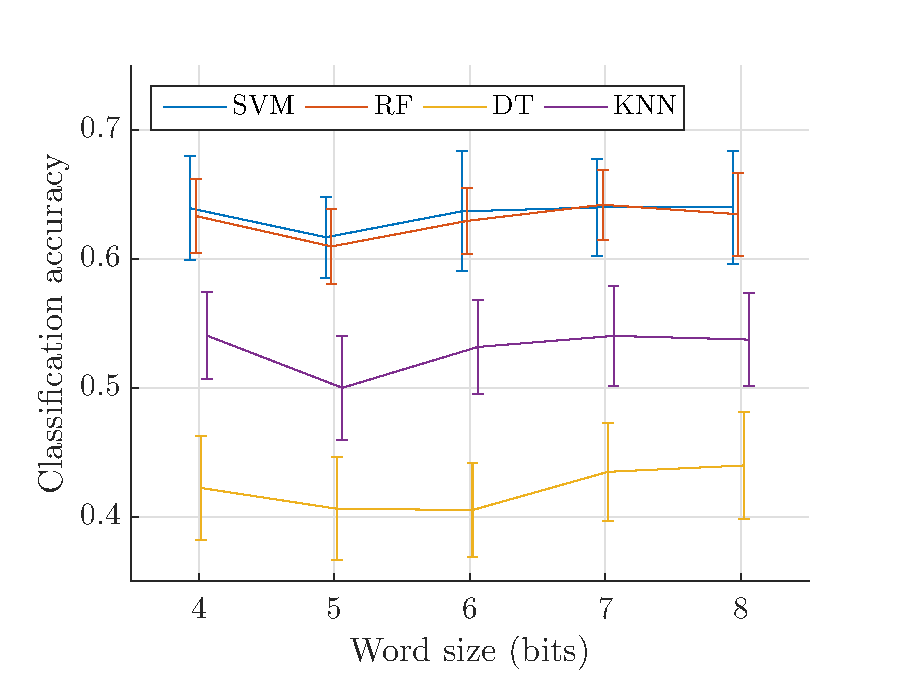
\includegraphics[width=0.5\textwidth]{figures/class_tob_q.eps}
	\caption{Classification accuracy with third-octave bands and varying word size.}
	\label{fig:class_tob_q}
\end{figure}

To further analyze both representations advantages, the confusion matrix is a reliable tool. It aims at providing information regarding class-by-class accuracy and misclassification rates. We thus compute these metrics for the SVM classifier, with predictions accumulated over the ten folds in test configuration. The analogous natures of the two descriptors is highlighted by close one-versus-one differentiation performances, with a slightly lower accuracy for third-octave bands on average. Both representations yield best results for the \textit{Gun shot} class with 88.2\% for third-octave cepstra and 86.6\% for Mel cepstra. Their poorest accuracy is on the \textit{Air conditioning} class with 32.0\% and 38.1\% respectively. However, a noticeable difference between them is that on the log-frequency scale the bandwidth of Mel filters narrows as frequency increases, while third-octave are evenly distributed. The effect of this can be seen between classes \textit{Drilling} and \textit{Jackhammer}. These sounds involve important low-frequency information which can generally differentiate them, leading third-octave descriptors to perform better. Conversely, using Mel-based cepstra improves globally \textit{Air conditioning} recognition as most of its defining components are situated in higher frequencies.\\

Both descriptor are thus found to have similar representational capabilities despite minor differences due to their respective designs.


\subsection{Inintelligibility}

The perceptual test \footnote{Decoded speech utterances for various conditions can be listened to at \url{https://felixgontier.github.io/cense-coder/}} then evaluates the impact of analysis frame rate on intelligibility using the average intelligibility score (AIS) given by the subjects and the intelligibility ratio (IR) computed as the number of correctly transcribed words versus the number of words in the spoken utterance.

The results of the perceptual test visible in Figure~\ref{fig:subj_int} confirm the qualitative evaluation of speech properties discussed in Section \ref{sec:inintelligibility}. Phonemes separation is indeed mandatory in order to ensure good intelligibility of speech. This implies an analysis frame rate significantly larger than the phonemes rate the considered language. A limit of about 10~Hz corresponding to a frame duration of 100~ms is observed, as the studied 8~Hz setting is found to be almost completely inintelligible. Very few words are understood correctly. We assume that the correctly identified words are a result of coincidentally adequate frame timings, \textit{i.e.} analysis frames matching the location of phoneme utterances for a short duration. Similarly, framing effects induced by the proposed processing scheme yielded errors for higher frame rates transcriptions and a globally lower perceptual intelligibility.\\


\begin{figure}[htbp]
	\centering
		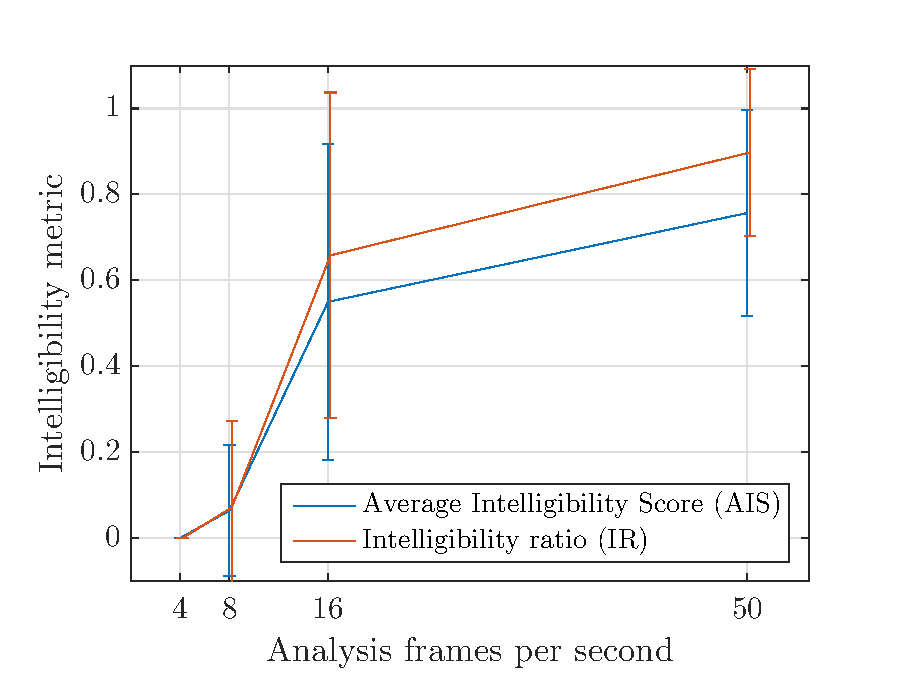
\includegraphics[width=0.5\textwidth]{figures/subj_int.eps}
	\caption{Normalized Average intellibility score (AIS) given by the subjects and the inteligibility ratio (IR) as a function of the frame rate. Inintelligibility appears at around 10~Hz, corresponding to the average duration of a phoneme.}
	\label{fig:subj_int}
\end{figure}

\section{Conclusion}

An audio encoding scheme has been described and motivated for use in a sensor grid approach to tackle the problem of large scale acoustic monitoring. It has been designed to transfer data from acoustic sensors to processing and storage servers in an efficient and effective manner. It relies on a lossy audio coding scheme designed to the guaranty the privacy of the citizens while retaining the needed amount of acoustic precision to compute standard acoustic descriptors and to allow the recognition of events of interest at a state of the art level of recognition accuracy.

It is based on a third octave spectral representation computed at an adjustable frame rate, encoded using an Huffman encoding scheme after logarithmic compression and differential encoding.

The proposed approach has the following benefits:
\begin{itemize}
	\item precision: the impact of the quantization step for 8 bits codewords is found to be very small (< 0.5dB) and thus:
	- do not impact the quality of the acoustics indicators.
	- enable the sound recognition with the same quality than directly from the spectrogram.
	\item efficiency: for fast and slow modes, the bitrate is respectively about 1.4~kbps and 0.4~kbps for the high precision mode
	\item privacy: at all operating modes, the reverted audio signal is found to be inintelligible according to a perceputal test.
\end{itemize}

The encoding scheme is designed to be easy to implement and to lead to an efficient data format for storage and sharing across the research community. To encourage its use for other research projects, an open source Matlab implementation of the coder is available.

%As those constraints are to some extent orthogonal, the proposed approach is flexible enough to balance rapidly between several modes of operations by changing a few parameters in an intuitive manner.


Future work will focus on the use of such a sensor grid approach as part of the cense project where its effectiveness will be assessed in field conditions. The usefulness of more sophisticated encoding paradigms in order to further improve bitrate efficiency should also be studied. Also, a more thorough investigation shall be performed on the inversion methods used to recover audio data from encoded data in order to ensure that the inintelligibility constraint is indeed not violated for fast settings.

\section{Acknowlegments}

The authors would like to thank Christophe d'Alessandro for fruitful discussion on speech intelligibilty.

%=====================================
% References, variant B: external bibliography
%=====================================
\externalbibliography{yes}
%\bibliography{your_external_BibTeX_file}
\bibliography{biblio}

%%%%%%%%%%%%%%%%%%%%%%%%%%%%%%%%%%%%%%%%%%
\end{document}
